\documentclass[10pt,a4paper]{article}
\usepackage[utf8]{inputenc}
\usepackage{amsmath}
\usepackage{amsfonts}
\usepackage{amssymb}
\usepackage{hyperref}
\usepackage{graphicx,longtable,mathrsfs,color}
\usepackage{epsfig,subfigure,placeins,float} % plots
\usepackage[usenames,dvipsnames]{xcolor} % colour
\title{Notes: Error on the Power Spectrum}
\author{Sahba Yahya}
\begin{document}

\maketitle


\section{Analytic solution }
\begin{eqnarray}\label{FIJ_DEV}
F_{ij}^*&=& V_{\rm sur} \int_{k_{min}}^{K_{max}} \frac{ 2 \pi k^2 dk}{2 (2 \pi)^3} \left[1+\frac{1}{nP}\right]^2
\end{eqnarray}

where,
\begin{eqnarray}
P(k,\mu)&=& R(\mu,k)P_{lin}(k) \left[\frac{g(z)}{g(z_{in})} \frac{(1+z_{in})}{(1+z)}\right]^2 b^2,\\
R(\mu,k)& =&1.\label{eq:Rsig}
\end{eqnarray}
and
\subsection{Survey Volume Formula}
\begin{equation}\label{eq:vsur1}
V_{\rm sur} =4 \pi c \,f_{\rm sky} \int^{z_{\rm min}}_{z_{\rm max}} dV, 
\end{equation}
$dV$ defined as:\[dV=  (1+z)^2D_A^2 \frac{c }{H_0} \frac{1}{h(z)} dz \]
where $h(z) = H(z)/H_0$. 
To convert from ${\rm Mpc}^3$ to ${\rm Mpc}^3 h^{-3}$ you need to multiply by $h^3$. The units for the $V_{\rm sur}$ is $h^{-3} {\rm Mpc}^3$.
\begin{equation}
V_{\rm sur} = 4 \pi c \,f_{\rm sky} \int^{z_{\rm min}}_{z_{\rm max}}  \frac{D_A^2(z)( 1+z)^2}{H(z)}  dz
\end{equation}
where 
\begin{equation}
f_{\rm sky} =   \left(\frac{\pi}{180}\right)^2 \frac{S_{\rm area }}{4 \pi}
\end{equation}
substituting the value of $dV$ and $f_{\rm sky}$ in Eq.~\ref{eq:vsur1}, then the $V_{\rm sur}$ could be written as:
\begin{equation}\label{Vsurvey}
V_{\rm sur} = \left(\frac{\pi}{180}\right)^2  \ S_{\rm area}\int^{z_{\rm min}}_{z_{\rm max}} ( 1+z)^2 D_A^2(z) \frac{c }{H_0} \frac{1}{h}  dz
\end{equation}
where $z_{\rm min} = 0. 9 $,  $z_{\rm max} = 1.1 $ and $S_{\rm area} = 30000 \  {\rm deg}^2$. 

Setting $ n \sim \infty$ 
\begin{equation}
F_{ij}^*= V_{\rm sur} \int_{k_{min}}^{K_{max}}  \frac{ 2 \pi k^2 dk}{2 (2 \pi)^3}
\end{equation}

solve the integral 
\begin{equation}\label{dp_ov_p}
F_{ij}^*= V_{sur} \frac{1}{ (24 \ \pi^2 )} \left[ k_{max}^3 -k_{min} ^3 \right]
\end{equation}

Arbitrary choices, $k_{min} = 0.001$, $k_{max} = 0.1$ and $V_{\rm sur} = 3{\rm e}10$ for z=1, and survey area is 30000 [deg$^2$]:

\begin{equation}
F_{ij}^* = 5.25512 \times 10^{-7}  V_{\rm sur}   = 8554,
\end{equation}
\begin{equation}
\frac{\delta P}{P} = \sqrt{(F_{ij}^*)^{-1}} = 0.011,
\end{equation}
Fig.~\ref{fig:cosmic_limit} shows $\frac{\delta P}{P}$ for $S_{rms} = 7.3$ and  the analytic solution proven above.
%====================================
\section{Euclid}

 Fig.~\ref{fig:cosmic_limit_Euclid_1} shows Euclid $\frac{\delta P}{P}$ produced using the definition in Bull et al 2014, not this figure shows produced with z =1, the bias = $ \sqrt{(1+z)}$ =1.41421, $k_{\rm max} = 0.16926\  h {\rm Mpc}^{-1}$, the survey volume has been calculated using Eq.~\ref{Vsurvey} and the Survey area is 15000 deg$^2$.



Fig.~\ref{fig:cosmic_limit_Euclid_2} shows the binned $k$ $\rm{Mpc}^{-1}$h. To check with Phil Bull results, we run camb with Plank's best fit parameters (see Fig.~ \ref{fig:pk_vs_k}):

\begin{verbatim}
# Planck best-fit parameters
cosmo = {
    'omega_M_0':        0.316,
    'omega_lambda_0':   0.684,
    'omega_b_0':        0.049,
    'N_eff':            3.046,
    'h':                0.67,
    'ns':               0.962,
    'sigma_8':          0.834,
    'gamma':            0.55,
    'w0':               -1.,
    'wa':               0.,
    'sigma_nl':         7.,
\end{verbatim}
%The surprising thing and I don't understand is the breakage on the non-binned $\delta p/p$ (the problem solved!)

%================================================
\section{Fractional error on DA and H}
Fig.~\ref{fig:lnda_lnH} shows the errors on $\sigma_H/H \%$ and  $\sigma_{D_A}/D_A \%$ using wiggles only method.



\begin{figure}
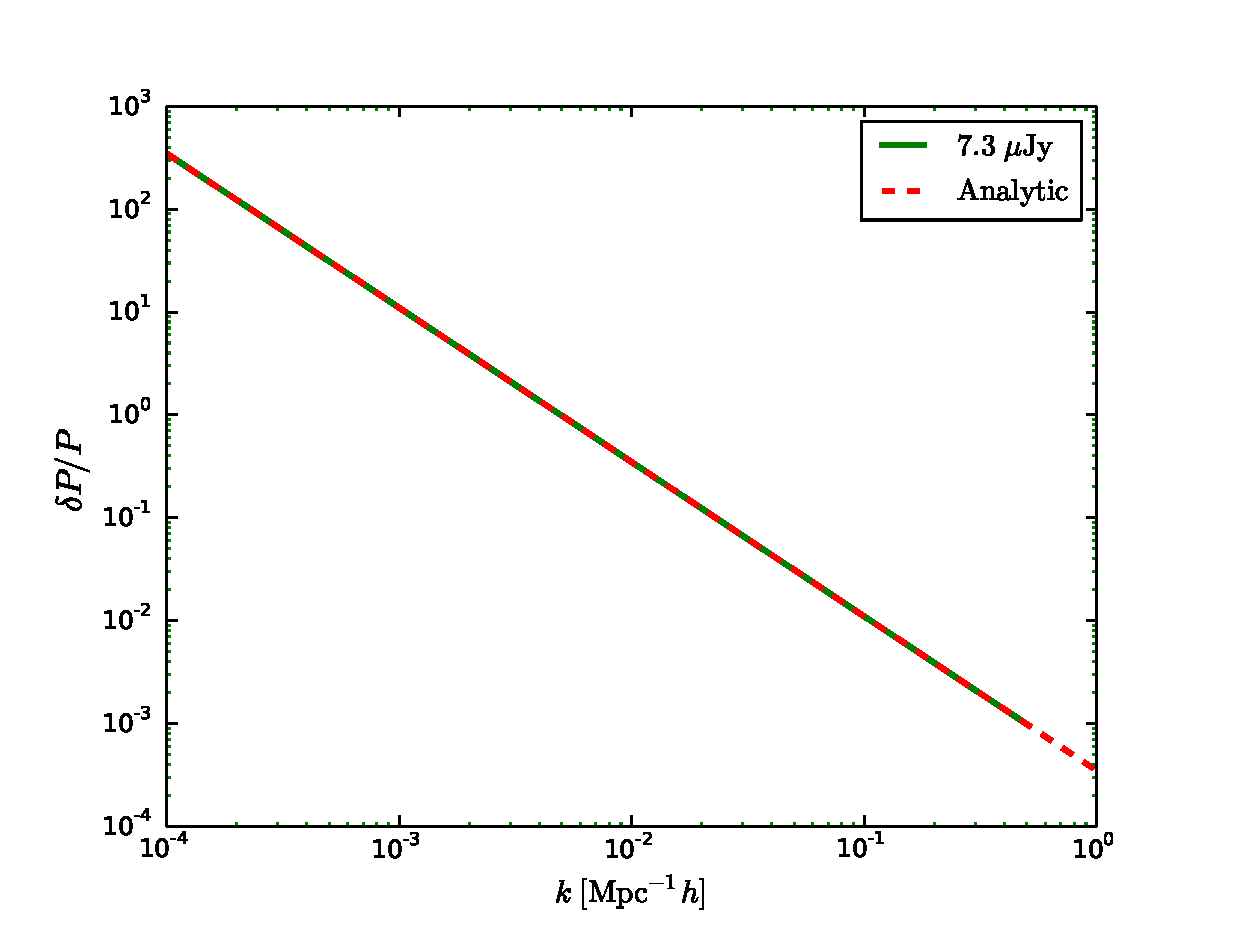
\includegraphics[width=0.7\textwidth]{deltaP_ov_p.eps}
\caption{The Figure shows $\delta P/P$ where n is very large (using Eq.~\ref{dp_ov_p}). The red dot point represent the analytic solution, for red-shift 1 and the corresponding bias=1.4.}
\label{fig:cosmic_limit}

\end{figure}



\begin{equation}
\left( \frac{\delta P}{P} \right)^2 =\left[ V_{\rm sur} \int_{k_{min}}^{K_{max}} \frac{ 2 \pi k^2 dk}{2 (2 \pi)^3} \left(1+\frac{1}{nP}\right)^2\right]^{-1}
\end{equation}



\begin{figure}
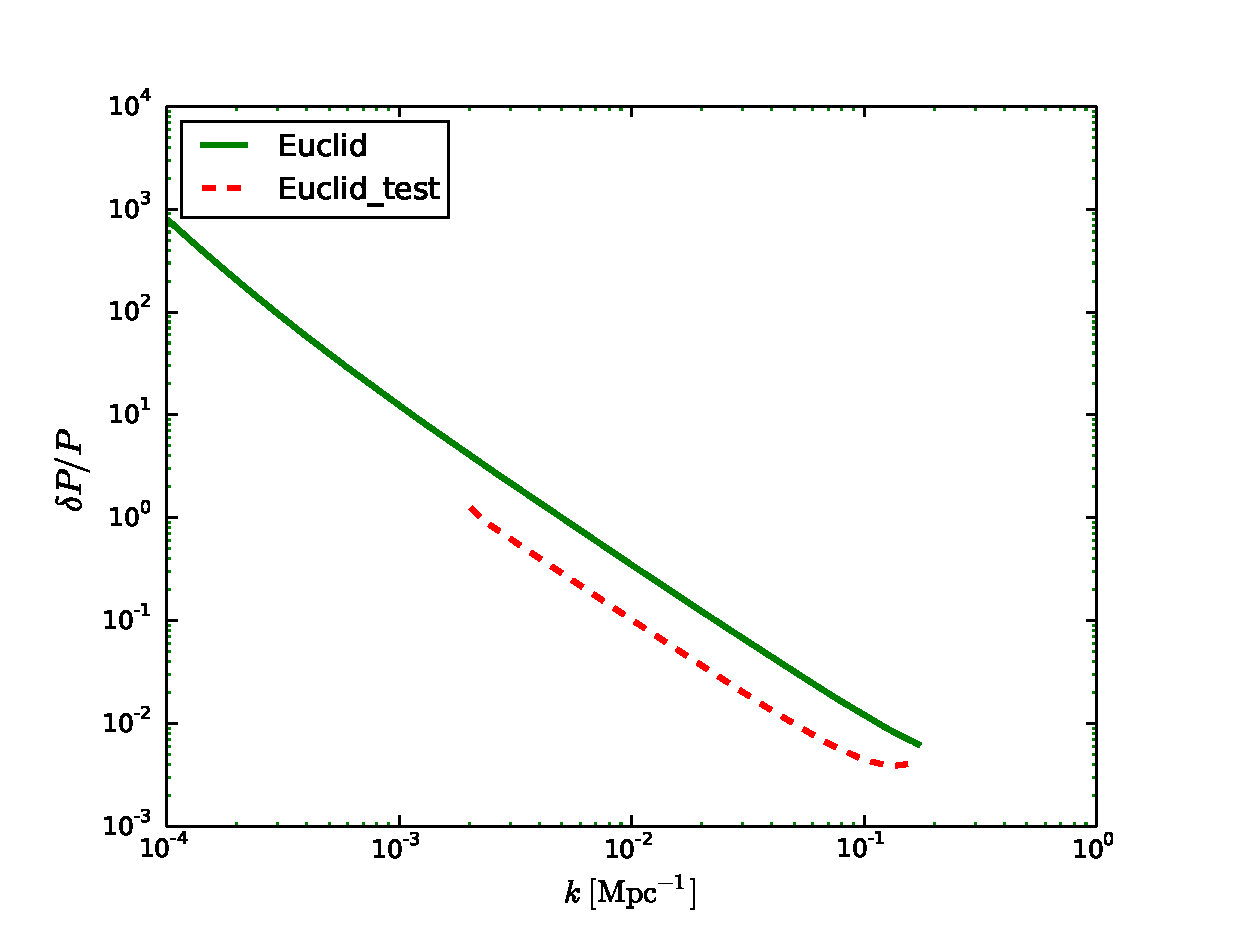
\includegraphics[width=0.8\textwidth]{deltaP_ov_p_Euclid_2.eps}
\caption{The Figure shows $\delta P/P$  for Euclid, for red-shift 1 and the corresponding bias=1.5.}
\label{fig:cosmic_limit_Euclid_1}
\end{figure}

\begin{figure}
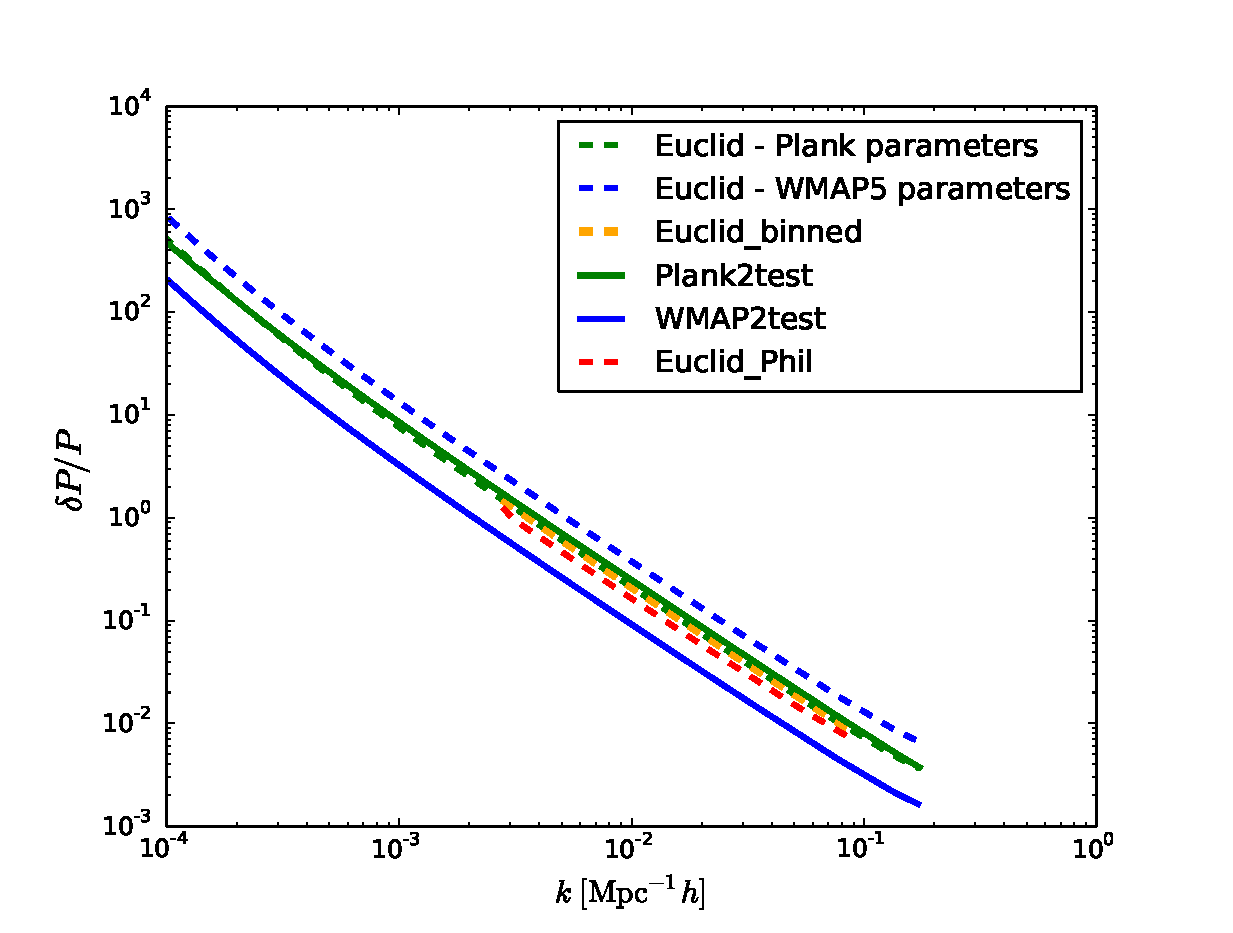
\includegraphics[width=0.7\textwidth]{deltaP_ov_p_Euclid.eps}
\caption{The Figure shows $\delta P/P$  for Euclid, for red-shift 1 and the corresponding bias=1.5. All the approached lie on top of each other except when we use the WMAP 5 parameters (blue).}
\label{fig:cosmic_limit_Euclid_2}
\end{figure}

\begin{figure}
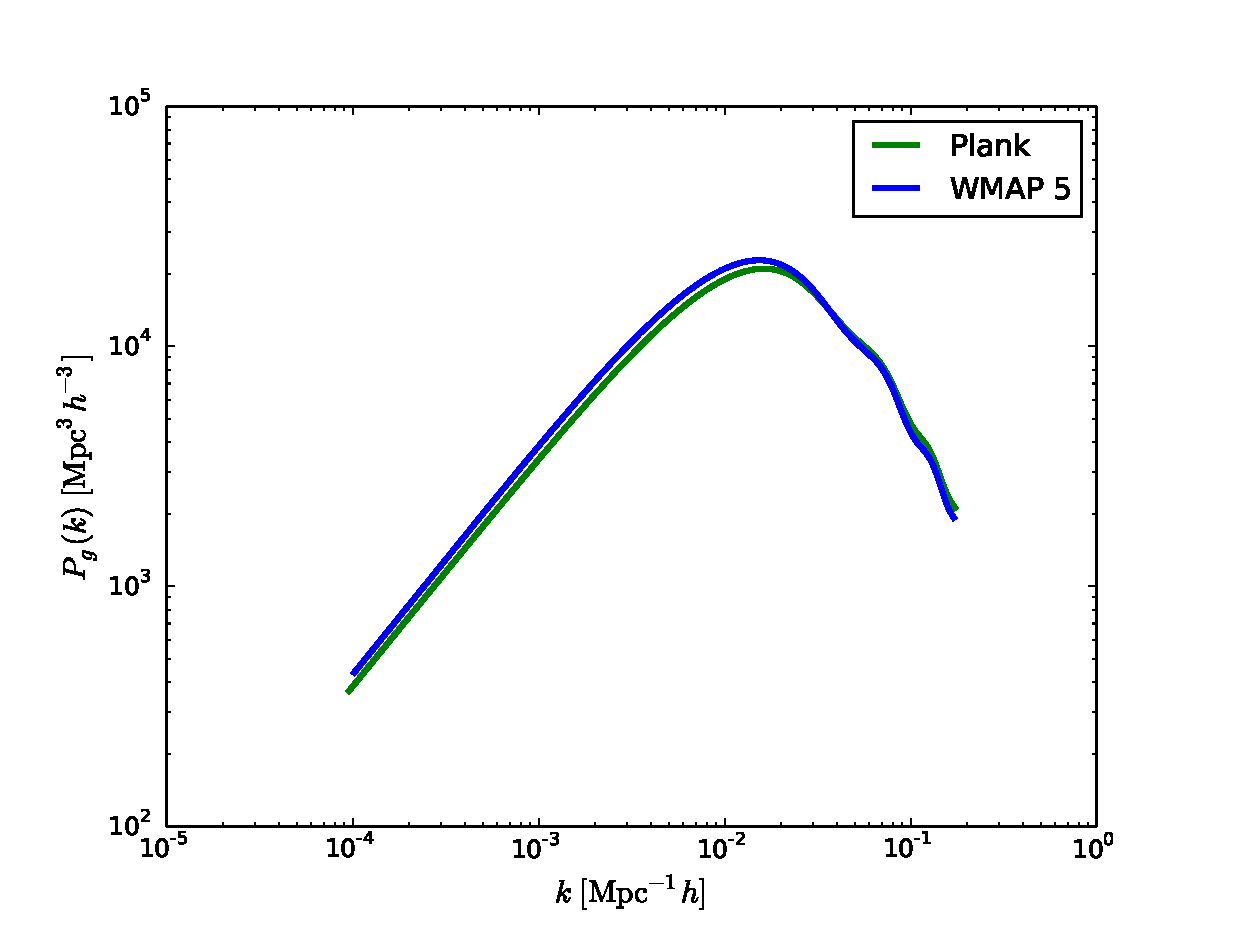
\includegraphics[width=0.7\textwidth]{pk.eps}
\caption{The power spectrum vs $k$ Mpc$h^{-1}$}
\label{fig:pk_vs_k}
\end{figure}
 

\begin{figure}
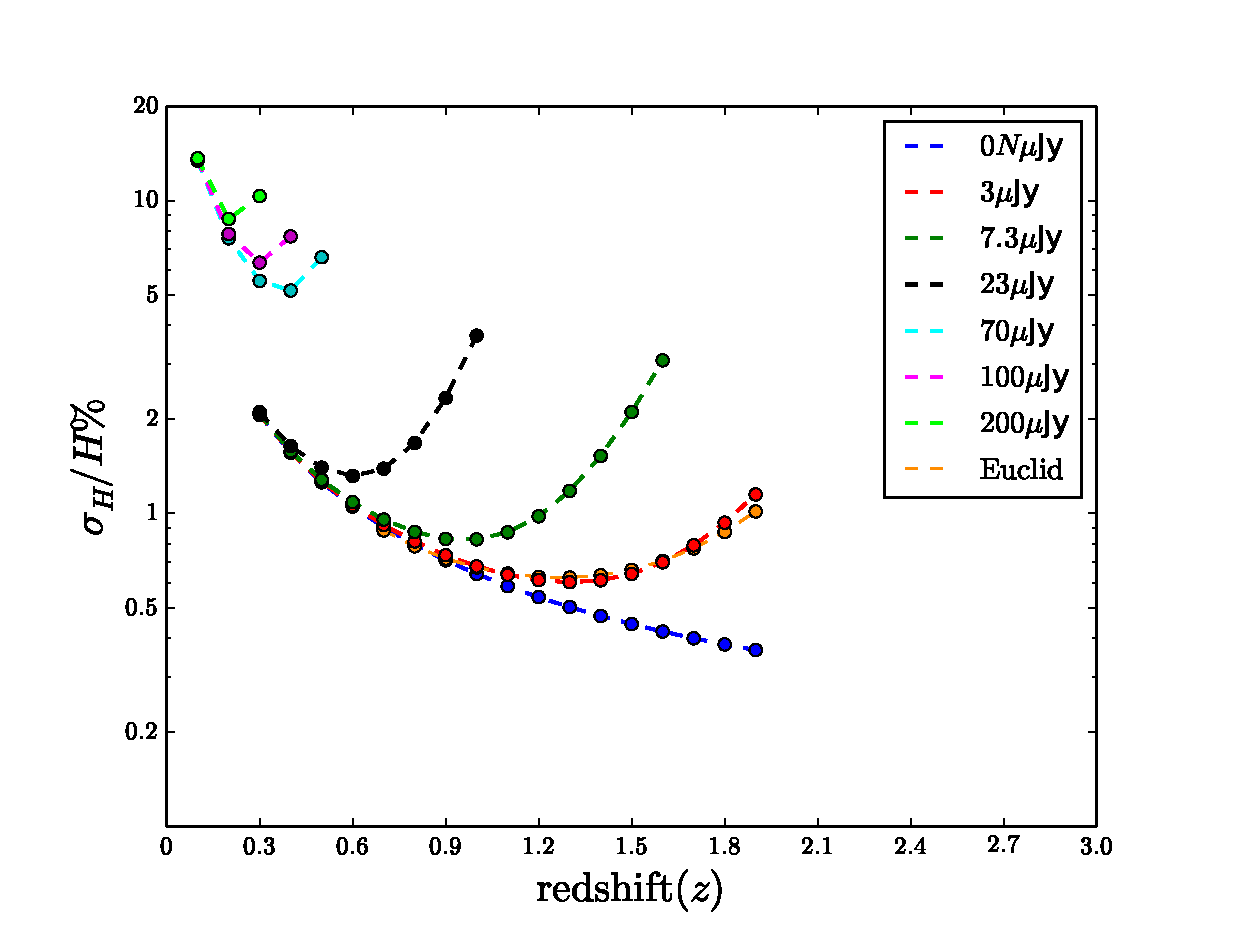
\includegraphics[width=0.7\textwidth]{output_lnH_mario_bias.eps}
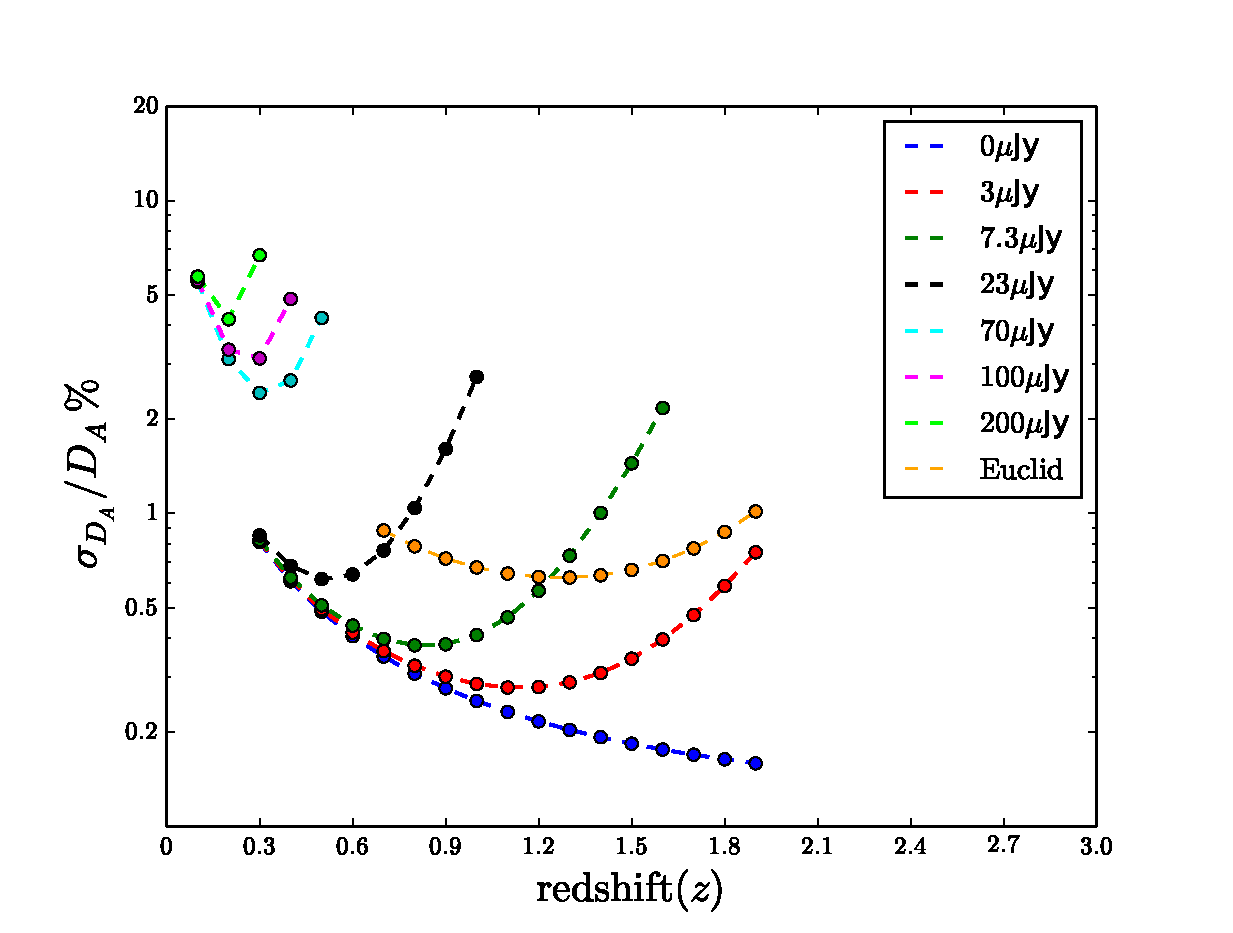
\includegraphics[width=0.7\textwidth]{output_lnda_mario_bias.eps}
\caption{The Figure shows $\sigma_H/H \%$ and $\sigma_{D_A}/D_A \%$  for SKA and  Euclid (orange).}
\label{fig:lnda_lnH}
\end{figure}


\section{Binning the Power spectrum}

Binning primary goal is to reduce the effects of minor observation errors. The original data values which fall in a given small interval (bin) replaced by a value usually in the middle of that interval. 

Combining Eq.~\ref{Vsurvey} and Eq.~\ref{dp_ov_p}  and replacing $k_{\rm min}$ and $k_{\rm max}$ by $k$ and $k+ \Delta k$ respectively, we get:
\begin{equation}\label{dp_ov_p}
F_{ij}^*= V_{sur} \frac{1}{ (24 \ \pi^2 )} \left[ k^3 -(k+ \Delta k) ^3 \right]
\end{equation}
\begin{equation}\label{dp_ov_p_deltak}
F_{ij}^*= V_{sur} \frac{1}{ (24 \ \pi^2 )} \left[ 2 k^3 + 3k^2  \Delta k  + 3 k \Delta k^2 + \Delta k^3 \right]
\end{equation}

Choosing the size and the width of the bin is essential, from Eq.~\ref{dp_ov_p_deltak}, choosing wider bins will make $\delta p/p$ smaller than choosing finer bins.

\section{Baryon Power spectrum}

\subsection{Produce the baryon power spectrum}
\begin{itemize}


\item[•] First we need to generate the P(k) for Plank parameters from camb with high resolution wiggles, to do that you have to modify camb with these option:
\begin{verbatim}
use_physical   = T
ombh2          = 0.022068
omch2          =0.12029E+00
 transfer_kmax           = 2
 transfer_k_per_logint   = 50 
\end{verbatim}
\item[•] Then we smooth the wiggles by putting $\Omega_b = 0.004$ (the lowest value camb can run without crashing).. and 
In this case we add the value of the  $\Omega_b$ to $\Omega_c$ then for this case, $\Omega_c({\rm new})= \Omega_c({\rm old}) + \Omega_b$.
\begin{verbatim}
use_physical   = T
ombh2          = 0.004
omch2          =0.142358E+00
 transfer_kmax           = 2
 transfer_k_per_logint   = 5
\end{verbatim}
\item[•] see Fig.~\ref{fig:pk_ov_pkref}.
\begin{figure}
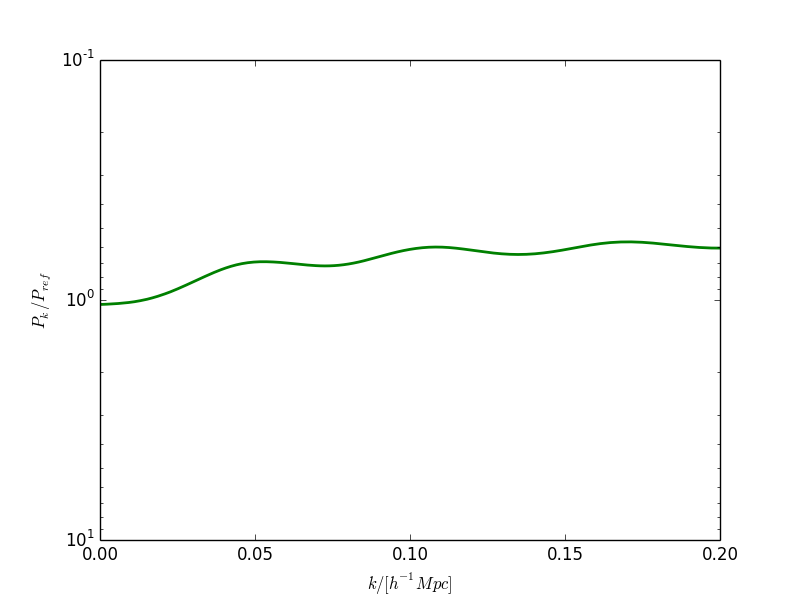
\includegraphics[width=0.8\textwidth]{Pb_vs_Pnobaryons_test.png}
\caption{The power spectrum P(k) over P(k) ref}
\label{fig:pk_ov_pkref}
\end{figure}
\end{itemize}

Using bao wiggles code,  the code smooth the power spectrum then subtract the smoothed from the original power spectrum, the results will give the BAO wiggles function. 
Then we can define the power spectrum:
\begin{equation}
P(k) = \left[1 + F_{\rm BAO}(k)\right] P_{\rm ref}(k)
\end{equation}


\begin{figure}
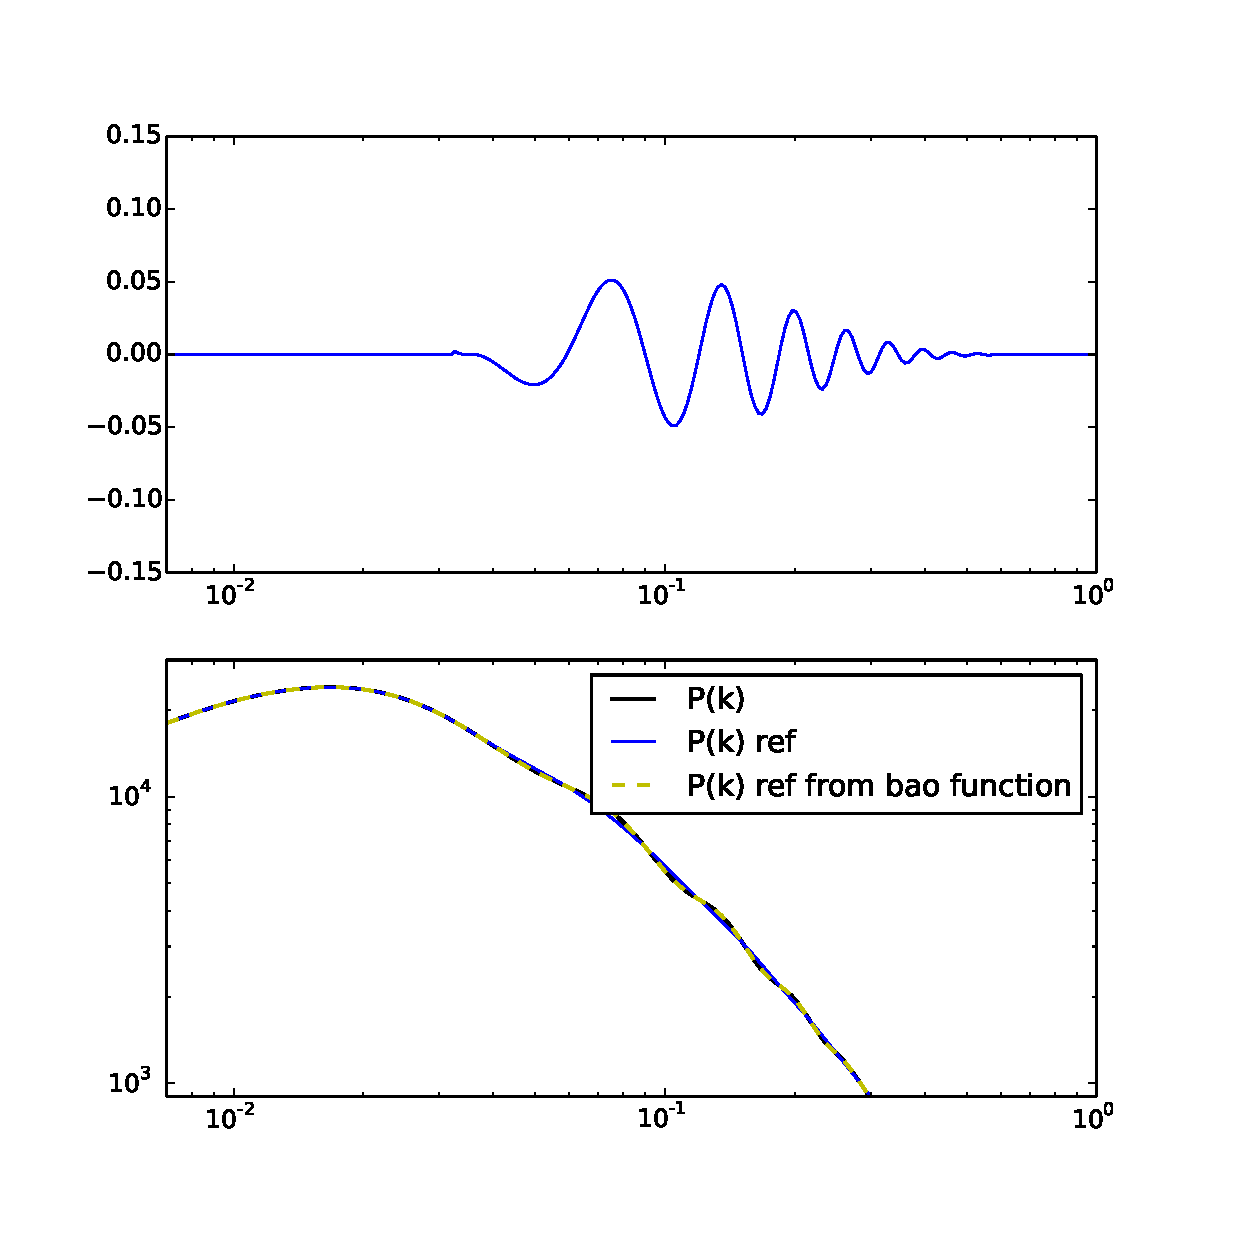
\includegraphics[width=1.0\textwidth]{test_wiggles_func.eps}
\caption{The power spectrum P(k), the smoothed power spectrum and the BAO(k)  function $F_{\rm BAO}(k)$ on the top panel. on the x-axis  k in $Mpc^{-1} h	 $, and on the y-axis the units are $Mpc^{3} h^{-3}$}
\label{fig:test_wiggles_func}
\end{figure}

\subsubsection{Numerical differentiation of $P_b(k)$}

As we describe the power spectrum in term of BAO function, the BAO function will be the wiggles only power spectrum. Then we can differentiate the function with respect to k.
we could use the finite difference method, its a common method to  approximation  the first and the second derivatives. The  defintion of the derivative of a function $f(a)$:

\begin{equation}
f'(a)  =\frac{ f(a+h) - f(a) }{h} - O(h)
\end{equation} 
where $h$ is the step size and $O(h)$ is the dominating error. This two point formula is good when the second derivative of the function is close to zero. 

It is better to use the three point formula to estimate the derivative of a function  such as such as  $a + bx^2$,  in case that some of x  values are negative.

\begin{equation}
f'(a) = \frac{f(a+h) - f(a-h)}{2 h} - \frac{h^3 f'''}{6} + O(h^3)
\end{equation}

More accurate method that we found is the Parabola method
 \url{http://mathfaculty.fullerton.edu/mathews//n2003/NewtonPolyMod.html}.
 
The method works as the following, stepping  through all the points from 2 to $n-1$. For each point (i) there is one on the left (i-1) and one on the right (i+1). We can draw an explicit parabola through these three points (just as we can draw a line through two points). The equation for a parabola is $y = A x^2+B x+C$, and for each point the do-loop finds the A, B and C for the parabola that runs through the point and the two on each side. The slope at the center point (i) is $ y' = 2 A x(i) + B$. Note that A, B and C are different for each step. This function has been tested on many functions $x^2$, $\exp(x)$ and $cos(x)$. the derivatives of those functions calculated using the Parabola method successfully. 

using this derivative we evaluate the numercial derivative of $\partial  F_{\rm BAO}(k)/ \partial k$, see Fig.~\ref{fig:diff_FBAO}

\begin{figure}
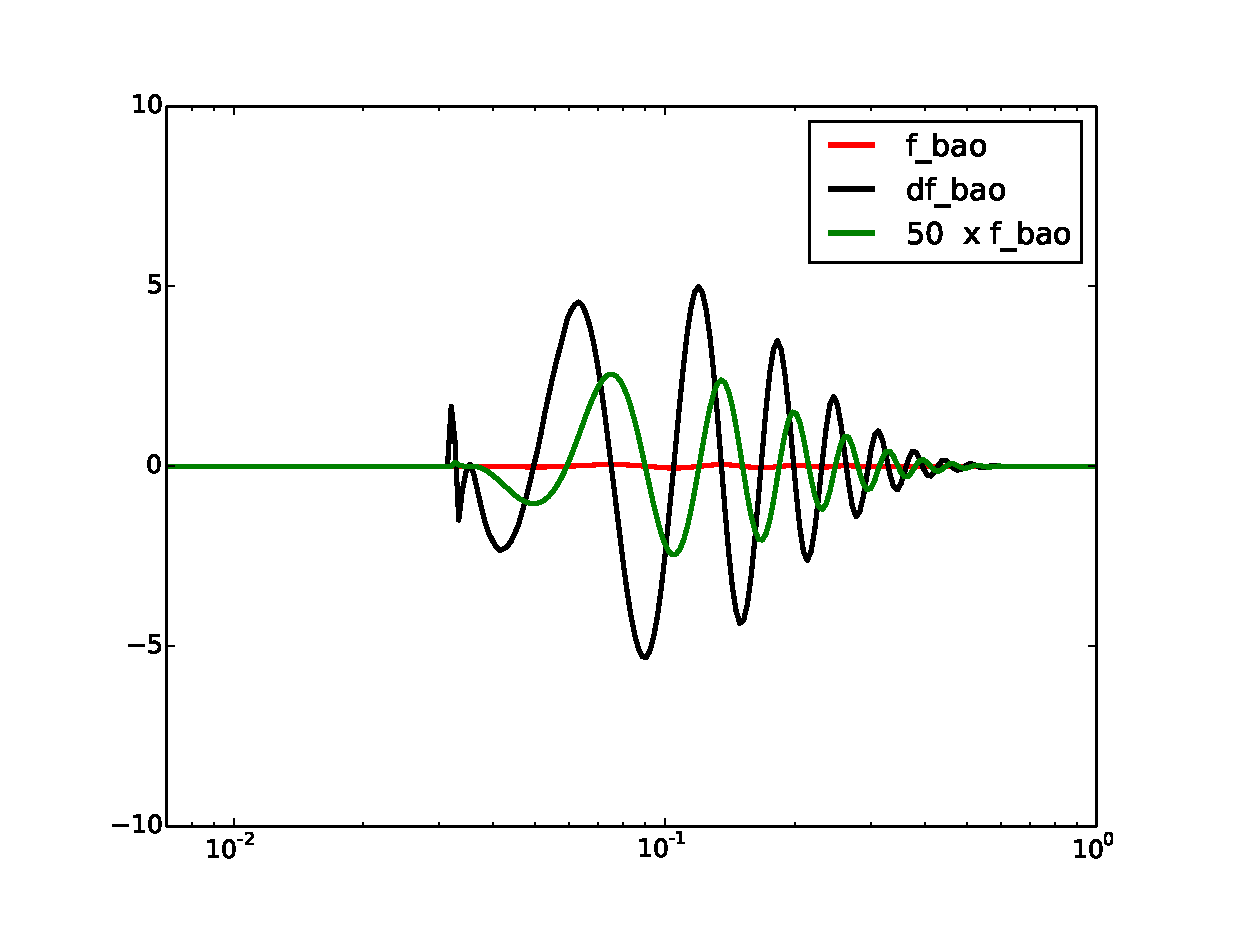
\includegraphics[width=0.7\textwidth]{derivative_of_fbao.eps}
\caption{Shows the function $F_{BAO}$ (red), $F_{BAO}$ multiplied by 50 (green) and the numerical derivative of $F_{BAO}$ with respect to k (black). }
\label{fig:diff_FBAO}
\end{figure}
\begin{figure}
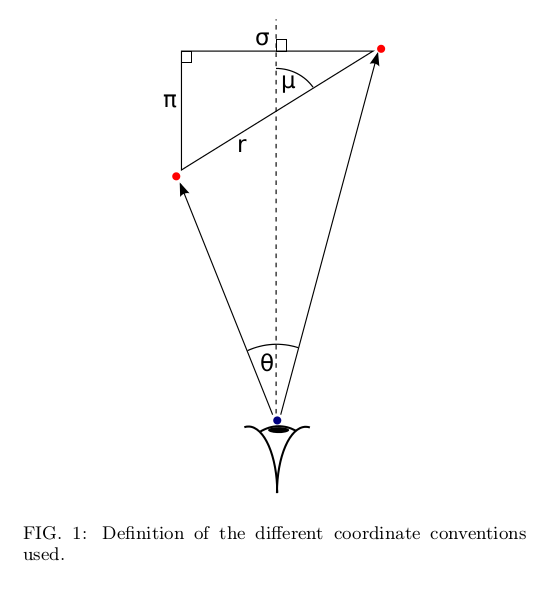
\includegraphics[width=0.7\textwidth]{mu_angle.png}
\caption{}
\label{fig:mu}
\end{figure}
\subsubsection{The analytic  differentiation of the $P_b(k)$ }

Lets define the basic quantities and parameters:
\begin{equation}
k ^2 = k_\parallel^2 + k_\perp^2
\end{equation}\label{eq:k}
\begin{eqnarray}
k_{\perp {\rm ref}} &=& \frac{k_{\perp} D_A (z) }{{D_A(z)}_{\rm ref}}   \\\nonumber
k_{\parallel {\rm ref} } &=& \frac{k_{\parallel} H(z)_{\rm ref}}{{H(z)}}
\end{eqnarray}\label{eq:perp_para}
where $k_{\parallel}$ and $k_{\perp}$ are the wave number along and across  the line of sight respectively,
and the total wave number is $k = \sqrt{k_\parallel^2 + k_\perp^2}$. The subscript ref means the reference cosmology and the ones without ref is the ones with true cosmology. not that $k_{\perp{\rm ref}}$ and $k_{\parallel {\rm ref}}$ are fixed.
$k_{\perp}$ and $k_{\parallel}$ are directly related to $\mu$:
\begin{equation}
k_{\perp}= k \sqrt{1 - \mu^2}  \;  \;\mbox{and} \;  \; k_{\parallel} = \mu^2 k
\end{equation}


Taking the derivative of k with respect to both quantities, H(z) and D(z):

\begin{eqnarray}
\frac{\partial k}{\partial D_A} &=& - \frac{ k_{\perp {\rm ref}}^2 D_A^2(z)_{\rm ref}}{D_A^3(z)}    \left[  \left(  k_{\perp {\rm ref} } \frac{D_A(z)_{\rm ref}}{D_A(z)}\right)^2 + k^2_{\parallel} \right]^{-\frac{1}{2}} \\\nonumber
\frac{\partial k}{\partial H} &=&    \frac{k_{\parallel {\rm ref}}^2}{H(z)_{\rm ref}^2} H(z)  \left[  \left(  k_{{\rm ref} \parallel} \frac{H(z)}{H(z)_{\rm ref}}\right)^2 + k^2_{\perp} \right]^{-\frac{1}{2}}
\end{eqnarray}\label{eq:dkdlogDa_H}

lets step back to check how we  formulate  the Fisher matrix:
\begin{eqnarray}\label{FIJ_DEV}
F_{ij}&=&\int_{-1}^{1}d\mu\int_{0}^{\infty}\frac{k^2dk}{8\pi} \frac{V_{\rm survey}}{\left[P^z+n^{-1}\right]^2}\nonumber \\
& \times & \left[\frac{\partial P_{b}}{\partial \ln (ks)} \right ]^2 
 \frac{\partial \ln (ks)}{\partial \theta_i}\frac{\partial \ln (ks)}{\partial \theta_j} .
\end{eqnarray}

If the fractional errors on $s_\perp^{-1}$ and  $s_\parallel$ is equivalent to measuring the fractional errors on $D_A/s$ and $Hs$ (where $s$ is the true physical value of the sound horizon.) 
\begin{equation}
 \frac{\partial \ln (ks)}{\partial \ln{s_\perp^{-1}}} = \mu^2 - 1
\end{equation}

\begin{equation}
\frac{\partial \ln (ks)}{\partial s_\parallel} = \mu^2
\end{equation}
where $\mu = \vec{k} . \vec{e}/k$ and $\vec{e}$ is the cosine the line of sight direction. see Fig.~\ref{fig:mu}

\begin{eqnarray}
 P_{ b} &=& \sqrt{8\pi^2} A_0 P_{0.2}\frac{\sin{ks}}{ks} \label{eq:gausilk} \\ \nonumber
 &&\times \exp{\left[-\left({k  \Sigma_{\rm S}}\right)^{1.4}-{k^2 \over 2} \left\{(1-\mu^2)\Sigma_\perp^2+\mu^2\Sigma_\parallel^2\right\} \right]},  
 \end{eqnarray}

\begin{eqnarray}
\frac{\partial P_{ b}}{\partial \ln (ks)} &=& \sqrt{8\pi^2} A_0 P_{0.2}\left(\cos{(ks)}  - \frac{\sin{(ks)}}{ks}\right) \label{eq:gausilk} \\ \nonumber
 &&\times \exp{\left[-\left({k  \Sigma_{\rm S}}\right)^{1.4}-{k^2 \over 2} \left\{(1-\mu^2)\Sigma_\perp^2+\mu^2\Sigma_\parallel^2\right\} \right]},  
 \end{eqnarray}

Numerically Fisher matrix will be:

\begin{eqnarray}\label{FIJ_DEV}
F_{ij}&=&\int_{-1}^{1}d\mu\int_{0}^{\infty}\frac{k^2dk}{8 \pi^2} \frac{V_{\rm survey}}{\left[P^z+n^{-1}\right]^2}\nonumber \\
& \times & \left[\frac{\partial [1+ F_{\rm BAO}(k)]P_{\rm ref}}{\partial \ln (ks)} \right ]^2 
 \frac{\partial \ln (ks)}{\partial \theta_i}\frac{\partial \ln (ks)}{\partial \theta_j} .
\end{eqnarray}




we can also rewrite the fisher matrix in this terms where $\theta_j$ and $\theta_i$ are replaced by the parameters we want to forecast for, $D_A$ and $H$:

\begin{eqnarray}\label{FIJ_re}
F_{ij}&=&\int_{-1}^{1}d\mu\int_{k_{\rm min}}^{k_{\rm max}}\frac{k^2 dk}{8\pi^2} \frac{V_{\rm survey}}{\left[P^z+n^{-1}\right]^2}\nonumber \\
& \times & \left[\frac{\partial F_{\rm BAO}(k)P_{\rm ref}}{\partial  k} \right ]\left[\frac{\partial  F_{\rm BAO}(k) P_{\rm ref}}{\partial  k} \right ]
 \frac{\partial k}{\partial \log D_A}\frac{\partial 
 k}{\partial \log H} .
\end{eqnarray}
assuming that the reference cosmology = true cosmology, and substituting equation \ref{eq:dkdlogDa_H},\ref{eq:k} and \ref{eq:perp_para}, the fisher matrix become:

\begin{eqnarray}
F_{ij}&=&\int_{-1}^{1}d\mu\int_{k_{\rm min}}^{k_{\rm max}}\frac{V_{\rm survey} \; k^2 dk}{8\pi^2} \left[\frac{ n(z)}{P(k)n(z)+1}\right]^2\nonumber \\
& \times & \left[\frac{\partial F_{\rm BAO}}{\partial k}\right]^2 \left[\frac{P(k)}{1+ F_{\rm BAO}}\right]^2 \left((\mu^2-1) k\right) \left(\mu^2 k \right)
\end{eqnarray}
where P(k) 
\begin{equation}
 P(k) = P_{\rm lin} \left[\frac{g(z)}{g(z_{in})}\right]^2  \left[\frac{(1+z_{in})}{(1+z)}\right]^2 R(\mu)^2  \; b^2 
\end{equation}
where
\begin{equation}
R(\mu) = 1 + \beta \mu
\end{equation}
\end{document}